
%(BEGIN_QUESTION)
% Copyright 2006, Tony R. Kuphaldt, released under the Creative Commons Attribution License (v 1.0)
% This means you may do almost anything with this work of mine, so long as you give me proper credit

Identifiser ``høy''- og ``lav''-portene på denne pneumatiske differansetrykktransmitteren, og forklar resonnementet ditt:

$$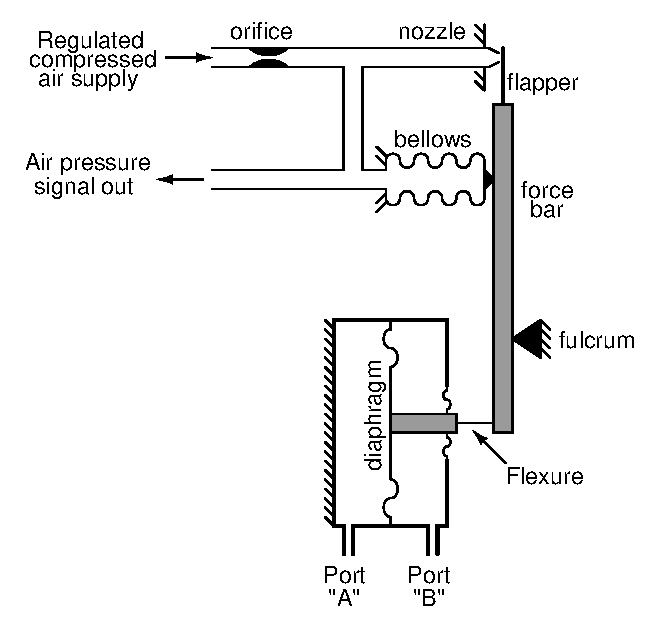
\includegraphics[width=15.5cm]{i00223x01.eps}$$

Forklar også hvordan transmitteren vil respondere på økende trykk på hver av de to portene, inkludert hvordan belgtilbakekoblingen fungerer.

\underbar{file i00223}
%(END_QUESTION)





%(BEGIN_ANSWER)

Port ``A'' er ``høy''-trykksporten på denne transmitteren, og port ``B'' er ``lav''-trykksporten.  Husk: økende trykk på ``høy''-porten gir økende signal ut fra transmitteren.  Omvendt gir økende trykk på ``lav''-porten et synkende signal ut fra transmitteren.

%(END_ANSWER)





%(BEGIN_NOTES)


%INDEX% Measurement, pressure: ``high'' versus ``low'' ports of a DP instrument

%(END_NOTES)
